\section{Relational convolutions with graphlet filters}\label{sec:relconv}

\subsection{Relational convolutions with discrete groups}
Suppose that we have a sequence of objects $(x_1, \ldots, x_n)$ and a relation tensor $R$ describing the pairwise relations between them, obtained by a MD-IPR layer $r(\cdot, \cdot)$ via $R[i,j] = r(x_i, x_j)$. The relational convolution operation we will define does two things: 1) extracts representations of the relational patterns within \textit{groups} of objects using pairwise relations, and 2) transforms the relation tensor back into a sequence of objects, allowing it be composed with another relational layer to compute higher-order relations. We begin by addressing the case when the groups are discrete and given.

Fix some filter size $s < n$, where $s$ is a hyperparameter of the relational convolution layer. One `filter' of size $s$ is given by the \textit{graphlet} $f_1 \in \mathbb{R}^{s \times s \times d_r}$. This is a `template' for the pairwise relations between $s$ objects. Note that the dimension of the relations in this filter matches that of the input relation tensor. Let $g \subset [n]$ be a group of $s$ objects among ($x_1, \ldots, x_n$) of the objects of size $s$. Suppose for now that $g$ is ordered (i.e., the group $(1, 2, 3)$ is different from the group $(2, 3, 1)$). Then, denote the relation sub-tensor associated to this group by $R[g] := [R[i,j]]_{i,j \in g}$. We define the `relational inner product' between this relation subtensor and the filter $f_1$ by
\begin{equation}
    \label{eq:relational_inner_prod_one_filt}
    \reliprod{R[g]}{f_1} \coloneqq \sum_{i,j \in g} \iprod{R[i,j]}{f_1[i,j]}_{\reals^{d_r}} = \sum_{i,j \in g} \sum_{k \in [d_r]} R[i,j,k] f_1[i,j,k].
\end{equation}
This is simply the standard inner product in the corresponding euclidean space $\mathbb{R}^{s^2 d_r}$. This quantity represents how much the relations within the objects in $g$ match the relations in the template $f_1$.


% Another relevant configuration is when the relation tensor $R$ is assumed to be symmetric (i.e.: pairwise relations are symmetric). In this case, filters can be restricted to be symmetric, and can now be identified with the smaller space $\{f \in \mathbb{R}^{s \times s \times r}: f[i,j] = f[j,i] \ \forall i,j \}$. The definition of the relational inner product can be simplified in this case to $\langle R[g], f_1 \rangle_R \coloneqq \sum_{i \leq j \in g} \langle R[i,j], f_1[i,j] \rangle$.

The relational convolution layer has $n_f$ filters (a hyperparameter). Denote the collection of filters by $\boldsymbol{f} = \paren{f_1, \ldots, f_{n_f}} \in \reals^{s \times s \times d_r \times n_f}$, which we call a \textit{graphlet filter}. We define the relational inner product of a relation subtensor $R[g]$ with a graphlet filter $\bm{f}$ as the $n_f$-dimensional vector consisting of the relational inner products with each individual filter,
\begin{equation}
    \label{eq:relational_inner_prod}
    \reliprod{R[g]}{\bm{f}} \coloneq \begin{pmatrix} \reliprod{R[g]}{f_1} \\ \vdots 
 \\ \reliprod{R[g]}{f_{n_f}} \end{pmatrix} \in \mathbb{R}^{n_f}.
\end{equation}
This vector summarizes various aspects of the relational pattern within a group, captured by several different filters\footnote{We have overloaded the notation $\reliprod{\cdot}{\cdot}$, but will use the convention that a collection of filters is denoted by a bold symbol (e.g., $\bm{f}$ vs $f_i$) to distinguish between the two forms of the relational inner product.}.Each filter corresponds to one dimension in the final relation-summarizing vector for the group $g$. This is reminiscent of convolutional neural networks, where each filter gives us one channel in the output tensor.

We can also define a symmetric variant of the relational inner product which is invariant to the ordering of the elements in $g$. This can be done by pooling over all permutations of $g$. In particular, we suggest max-pooling and average-pooling, although any set-aggregator would be valid. We denote the permutation-invariant relational inner product by $\iprod{R[g]}{f_1}_{\mathrm{rel}, \mathrm{sym}}$,
\begin{equation}\label{eq:symmetric_relational_inner_prod}
    \iprod{R[g]}{\bm{f}}_{\mathrm{rel}, \mathrm{sym}} \coloneq \mathrm{Pool}\paren{\set{\reliprod{R[g']}{\bm{f}} \colon g' \in g!}},
\end{equation}
\noindent where $g!$ denotes the set of permutations of the group $g$. Recall that each $\iprod{R[g']}{\bm{f}}_{\mathrm{rel}}$ is $n_f$-dimensional, and the pooling is done independently for each dimension.

For a given group $g \subset [n]$, the relational inner product with a graphlet filter, $\iprod{R[g]}{\bm{f}}_\mathrm{rel}$, gives us a vector summarizing the relational patterns inside that group. We aim to get a sequence of objects which each describes the relational patterns within each group of interest. Let $\calG$ be a set of groupings of the $n$ objects, each of size $s$. The relational convolution between a relation tensor $R$ and a relational graphlet filter $\bm{f}$ is the sequence of relational inner products with each group in $\calG$,
\begin{equation}
    \label{eq:relational_convolution}
    R \ast \bm{f} \coloneq \left( \reliprod{R[g]}{\boldsymbol{f}} \right)_{g \in \calG} \equiv \left(z_1, \ldots, z_{\abs{\calG}}\right) \in (\mathbb{R}^{n_f})^{\abs{\calG}}
\end{equation}
We assume that $\calG$ is given (i.e., a pre-specified hyperparameter of the relational convolution operation). If some prior information is known about reasonable groupings, this can be encoded in $\calG$. When $n$ is small and no prior information is available, a reasonable choice might be the the set of all combinations of size $s$. When $n$ is large, considering all combinations will be intractable. %One solution is to consider a random sample of combinations. 
In the next subsections, we consider the problem of \textit{differentiably learning} the relevant groups.

% In the above, we either consider all possible groups or we somehow assume that the relevant groups $\calG$ are known and given. We may also wish to \textit{learn} the relevant groups.

\begin{figure}
    \vskip-10pt
    \centering
    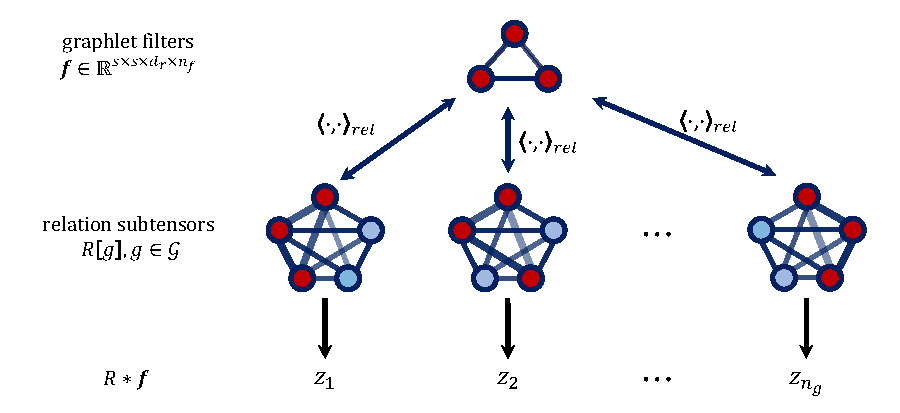
\includegraphics[width=0.9\textwidth]{figs/relconv_figs_updated.pdf}
    \caption{A depiction of the relational convolution operation. A graphlet filter $\bm{f}$ is compared to the relation subtensor in each group of objects, producing a sequence of vectors summarizing the relational pattern within each group. The groups can be differentiably learned.
    }\label{fig:relconvdiagram}
\end{figure}
% AWNI: [TODO] UPDATE THIS FIGURE. REMOVE OLD DEPICTION OF "SOFT GROUPS"

\subsection{Relational convolutions with group attention}

In the above formulation, the groups are `discrete'. Having discrete groups can be desirable for interpretability, if the relevant groupings are known a priori or if considering every possible grouping is computationally and statistically feasible. However, if the relevant groupings are not known, then considering all possible combinations results in a rapid growth of the number of objects at each layer.
% Besides being computationally intractable, considering every possible grouping may be unnecessary and may make learning more difficult.

In order to address these issues, we propose \textit{explicitly modeling groups}. This allows us to control the number of objects in the output sequence of a relational convolution operation such that only relevant groups are considered. We propose modeling groups via an \textit{attention} operation.

Consider the input $X = \paren{x_1, \ldots, x_n},\, x_i \in \reals^d$. Let $n_g$ be the number of groups to be learned and $s$ be the size of the graphlet filter (and hence the size of each group). These are hyperparameters to the model. We learn $n_g \times s$ group query vectors $Q = \{q_{i}^{g}\}_{g \in [n_g], i \in [s]}$. That is, for each group $g \in [n_g]$, we learn $s$ queries which will be used to retrieve a group of size $s$ via attention. The $i$-th object in the $k$-th group is retrieved via an attention operation as follows,
\begin{equation}\label{eq:group_attn}
    \begin{aligned}
        \bar{x}_{i}^{g} &= \sum_{j = 1}^{n} \alpha_{ij}^{g} x_j, \ &&g \in [n_g],  i \in [s]\\
        \alpha_{ij}^{g} &= \frac{\exp\paren{\beta \iprod{q_i^g}{\mathtt{key}(x_j)}}}{\sum_{k = 1}^{n}{\exp\paren{\beta \iprod{q_i^g}{\mathtt{key}(x_k)}}}}, \ &&k \in [n_g], i \in [s], j \in [n]
    \end{aligned}
\end{equation}
where $\bar{x}_{i}^{g}$ is the $i$-th object retrieved in the $g$-th group, $q_{i}^{g}$ is the query for retrieving the $i$-th object in the $g$-th group, $\mathtt{key}(x_j)$ is the key associated with the object $x_j$, and $\beta$ is a scaling parameter. % AWNI: mention $\beta$ learnable? vs fixed to 1/sqrt(d_k).

The $\mathtt{key}$ for each object is computed as a function of its position, features, and/or context. For example, to group objects based on their position, the key can be a positional embedding, $\mathtt{key}(x_i) = PE_i$. To group based on features, the $\mathtt{key}$ can be a linear projection of the object's feature vector, $\mathtt{key}(x_i) = W_k x_i$. To group based on both position and features, the $\mathtt{key}$ can be a sum or concatenation of the above. Finally, groups can also be modeled based on contextual information by computing keys after a self-attention operation, allowing objects to be grouped based on the context in which they occur.

\Cref{eq:group_attn} can be computed in parallel with an `einsum' operation in $\calO(n \cdot n_g \cdot s \cdot d)$ operations. When the hyperparameters of the model are fixed, this is linear in the sequence length $n$.

The relation subtensor $\bar{R}[g] \in \reals^{s \times s \times d_r}$ for each group $g \in [n_g]$ is then computed using a shared MD-IPR layer $r(x, y)$,
\begin{equation}
    \bar{R}[g] = \bra{r(\bar{x}_{i}^{g}, \bar{x}_{j}^{g})}_{i,j \in [s]}.
\end{equation}
This computation can be carried out in parallel via efficient matrix multiplication with $\calO(n_g \cdot s^2 \cdot d_r \cdot d_{\mathrm{proj}})$ operations. Note that This does not scale with the number of objects in the input, and is only a function of the hyperparameters of the model. Moreover, typically, the filter size $s$ is chosen to be of fixed order with respect to the number of objects $n$ (e.g., fixed to $3$ or $5$, as in CNNs).

The relational convolution is computed as before via,
\begin{equation}
    \bar{R} \ast \bm{f} \equiv \paren{\reliprod{\bar{R}[g]}{\bm{f}}}_{g \in [n_g]}.
\end{equation}

Overall, relational convolution with group attention can be summarized as follows: 1) learn $n_g$ groupings of objects, retrieving $s$ objects per group; 2) compute the relation tensor of each group using a MD-IPR module; 3) compute a relational convolution with a learned set of graphlet filters $\bm{f}$, producing a sequence of $n_g$ vectors each describing the relational pattern within a (learned) group of objects.

\textbf{Entropy regularization.} The group attention scores in~\Cref{eq:group_attn} are ideally close to discrete assignments. That is, the vector $\alpha_{i,\cdot}^{g} \in \Delta^{n}$ is ideally a one-hot vector for each $g \in [n_g],\, i \in [s]$. To encourage the model to learn more structured group assignments, we add an entropy regularization to the loss function, $\calL_{\mathtt{entr}} = \frac{1}{n_g \cdot s} \sum_{g, i} H(\alpha_{i,\cdot}^{g})$, where $H(\alpha_{i,\cdot}^{g}) = - \sum_{j} \alpha_{ij}^{g} \log(\alpha_{ij}^g)$ is the Shannon entropy. As a heuristic, this regularization can be scaled by $\sim \log(\mathtt{n\_classes}) / \log(n)$ so that it doesn't dominate the underlying task's loss.

\textbf{Computing input-dependent queries sequentially.} In the simplest case, the query vectors $Q$ are simply learned parameters of the model, representing a fixed criterion for selecting the $n_g$ groups. The queries can also be produced in an input-dependent manner. Concretely, the query vectors can be produced sequentially by an LSTM with each retrieved object fed back into the LSTM so that it can produce the next query according to the groups selected so far. I.e., $q_i^g \gets \mathrm{LSTM}(h_{i-1}, \bar{x}_{i-1}^g)$.